\documentclass[12pt]{book}
\usepackage{graphicx}
\usepackage{subfig} % make it possible to include more than one captioned figure/table in a single float
\usepackage[utf8]{inputenc}
\usepackage{hyperref}
\usepackage[intlimits]{amsmath}
\usepackage{amssymb}
\usepackage{tkz-euclide}
\usepackage{tikz}
\setlength{\oddsidemargin}{15.5pt} 
\setlength{\evensidemargin}{15.5pt}
\pretolerance=2000
\tolerance=3000
\renewcommand{\figurename}{Figura}
\renewcommand{\chaptername}{Cap\'{i}tulo}
\renewcommand{\contentsname}{\'{I}ndice}
\renewcommand{\tablename}{Tabla}
\renewcommand{\bibname}{Bibliograf\'{i}a}
\renewcommand{\appendixname}{Ap\'endices}


\begin{document}

Representación de B1422+231

\begin{figure}[!h]
 \centering
 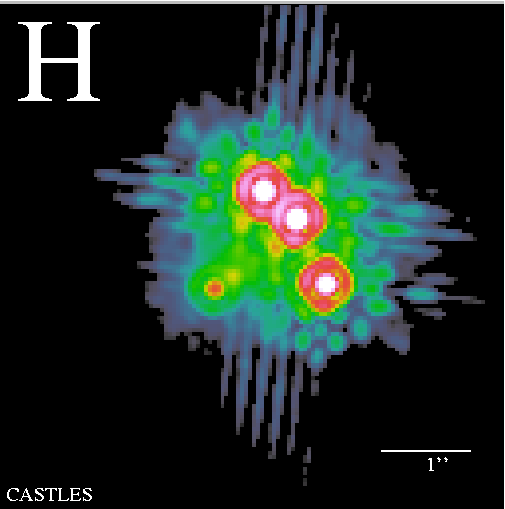
\includegraphics[scale=0.4]{B1422H.png}
 \caption{\emph{Imagen de http://www.cfa.harvard.edu/castles/Postagestamps/Gifs/Fullsize/B1422H.gif}}
 \label{Fig: 1}
\end{figure}

Imagen(nx=1000) obtenida con una fuente de anillos circulares concéntricos (ny = 200) a traves de una SIS (gamma = 0.6, x01 = -0.10, x02 = -0.20)

\begin{figure}[!h]
 \centering
 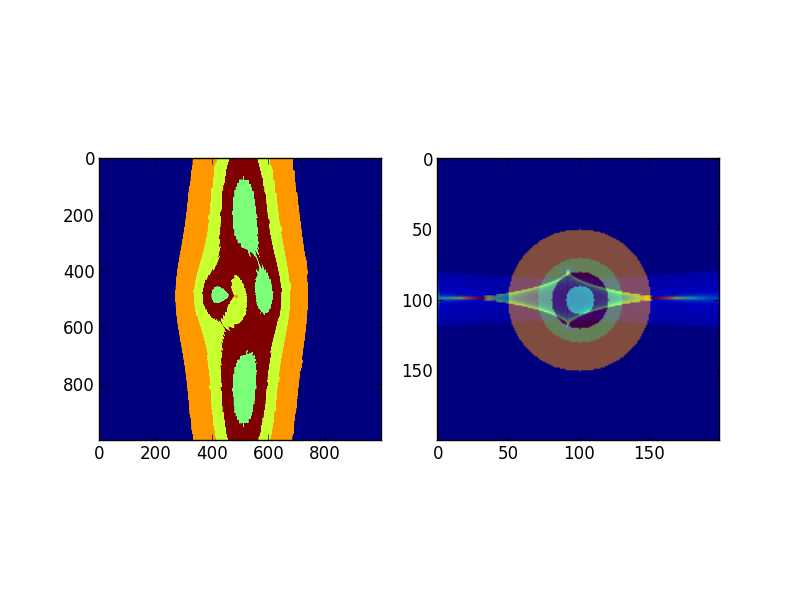
\includegraphics[scale=0.4]{b1422h-iso.png}
 \caption{\emph{xl=4,yl=4}}
 \label{Fig: 1}
\end{figure}

Imagen de una fuente (hubble deep field) a traves de una lente gravitacional(esfera singular isoterma)
\begin{figure}[!h]
 \centering
 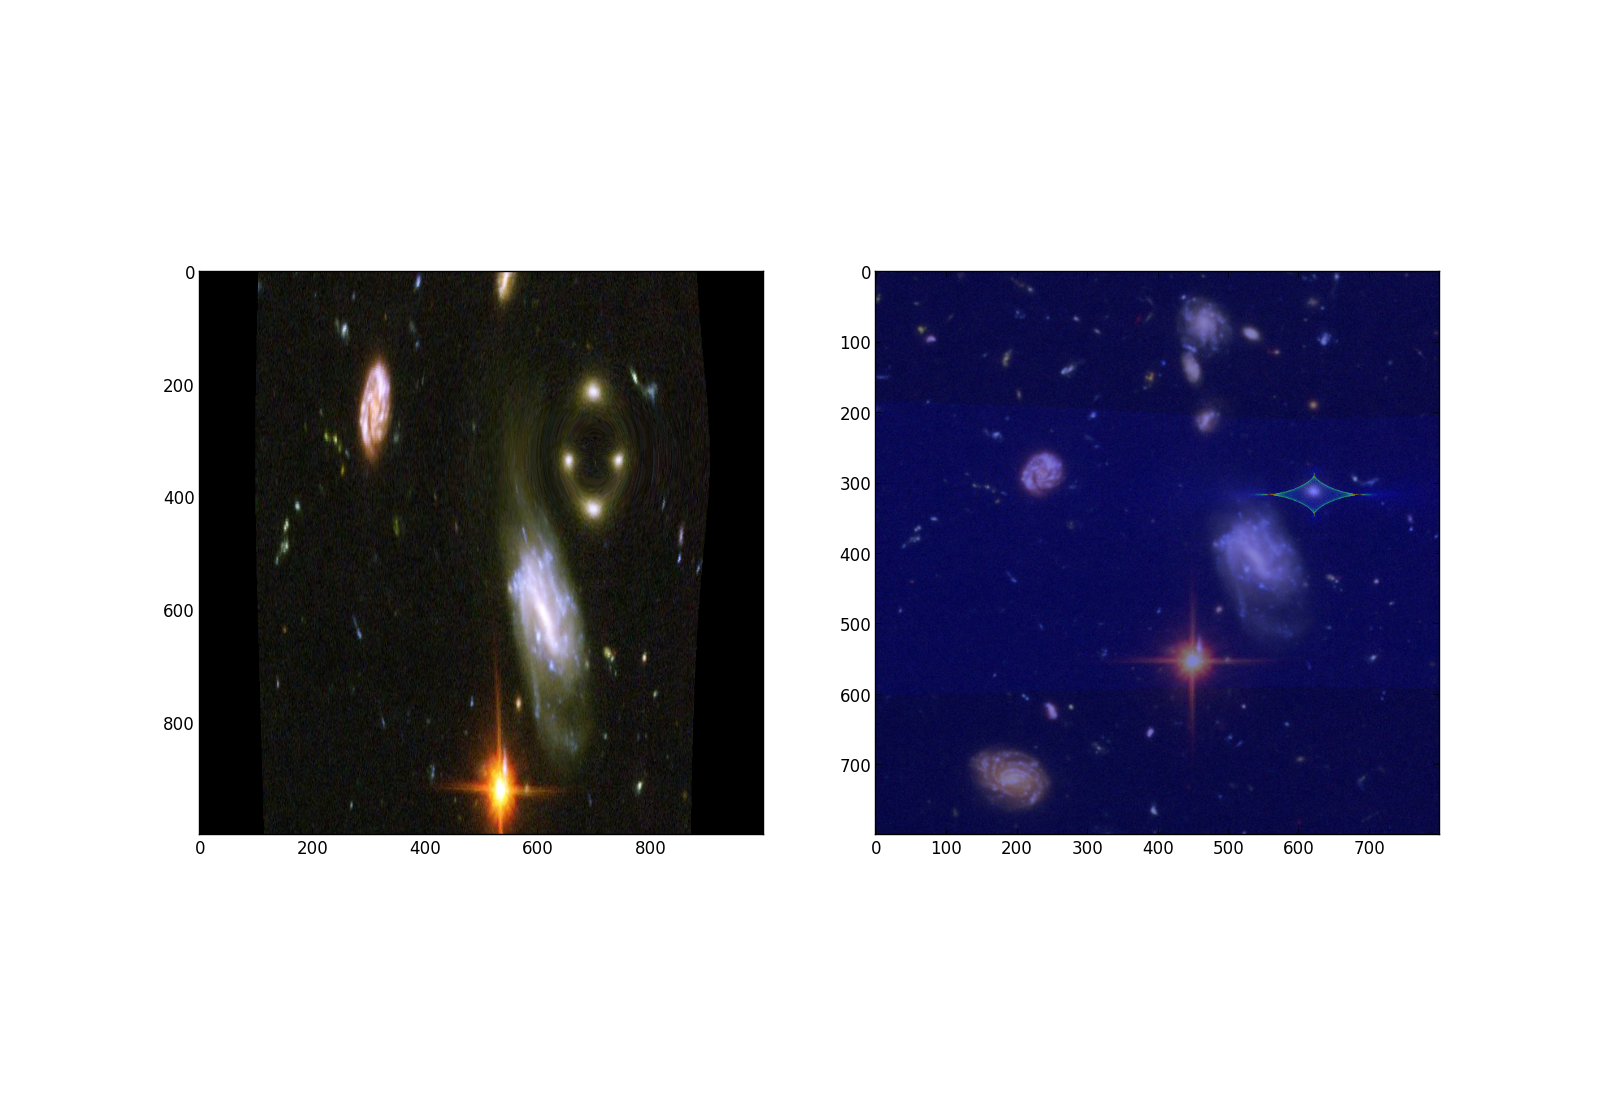
\includegraphics[scale=0.4]{hubble1.png}
 \caption{\emph{SIS(gamma=0.5,x01=-2.76,x02=3.15),ny=800,nx=1000,xl=8,yl=8}}
 \label{Fig: 2}
\end{figure}


Mapa de magnificación en el caso de un sistema binario
\begin{figure}[!h]
 \centering
 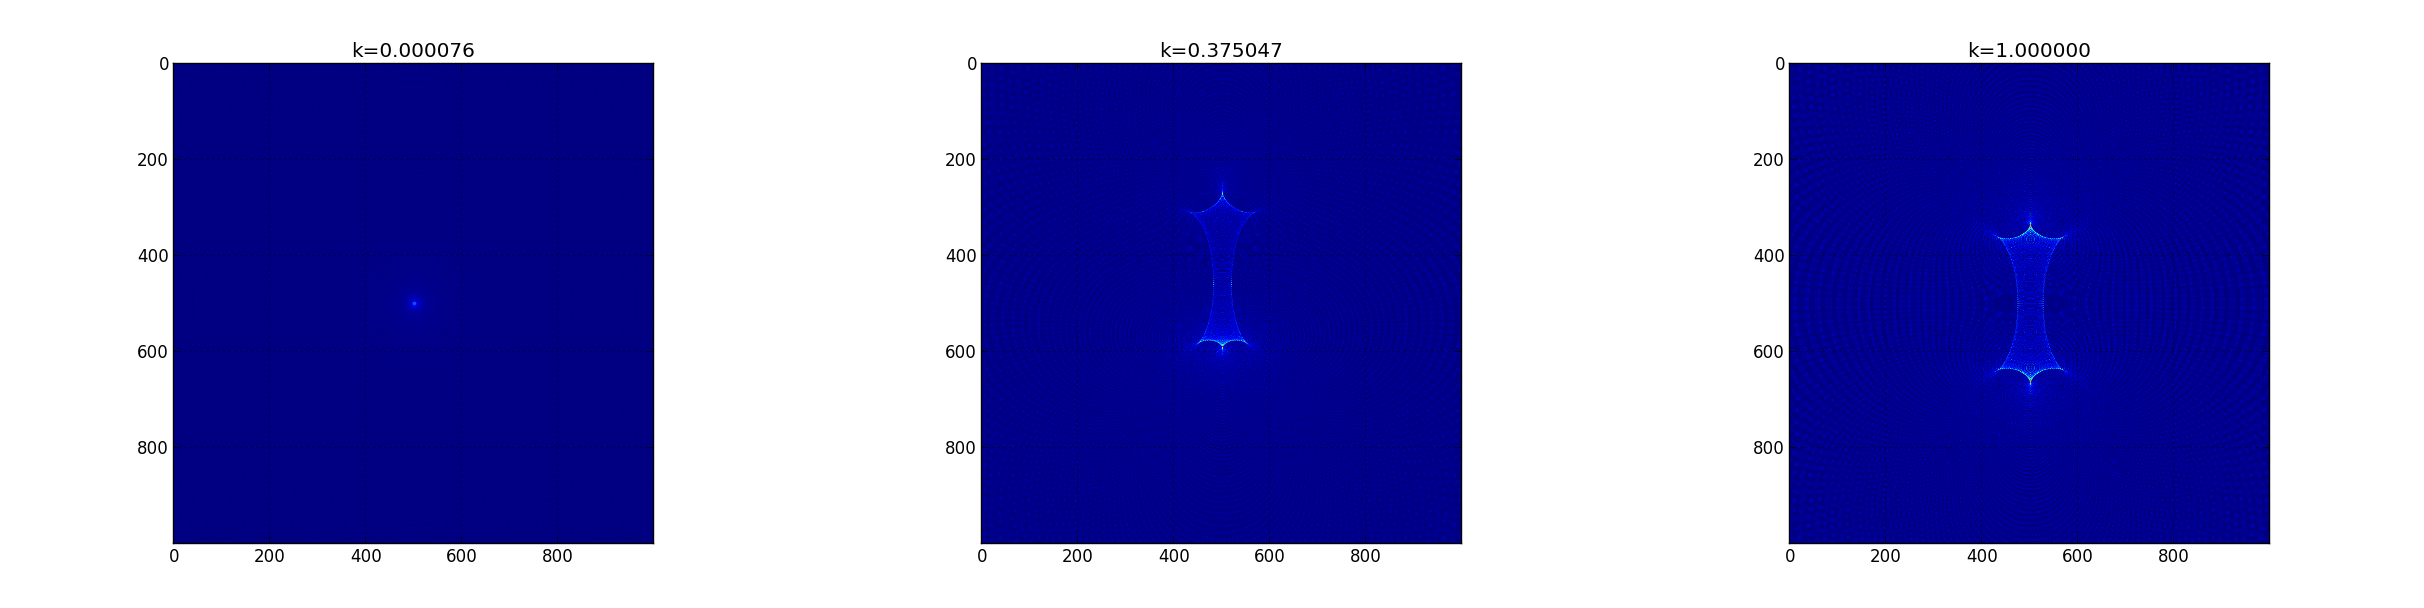
\includegraphics[scale=0.2]{mag_bs.png}
 \caption{\emph{k=M1/M2}}
 \label{Fig: 3}
\end{figure}


Mapa de magnificación en el caso de un sistema binario(estrella-planeta)
M1/M2 = 7.6 * 10 ** (-5), a = 1.61, ny = 100, nx = 30000, xl = 1, yl = 0.00025 
\begin{figure}[!h]
 \centering
 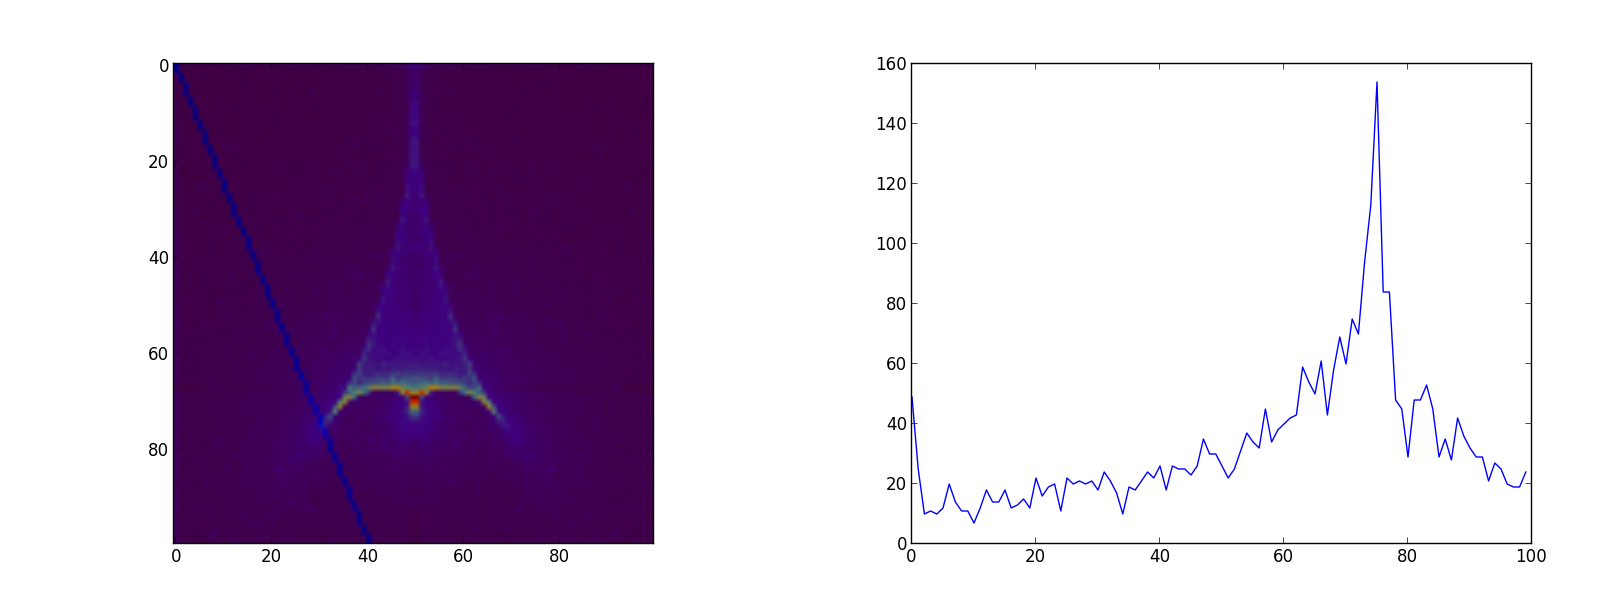
\includegraphics[scale=0.3]{bscurve.png}
 \caption{\emph{A la derecha el corte del mapa de magnificacion al largo de la curva:  y =  abs(tan(theta) * x + u0 * (cos(theta) + sin(theta) * tan(theta))), u0 = 0.359, theta = 2.756 rad  }}
 \label{Fig: 4}
\end{figure}

Imagenes de una fuente de anillos concéntricos (cruzando la caustica) y mapas de magnificación correspondientes
\begin{figure}[!h]
 \centering
 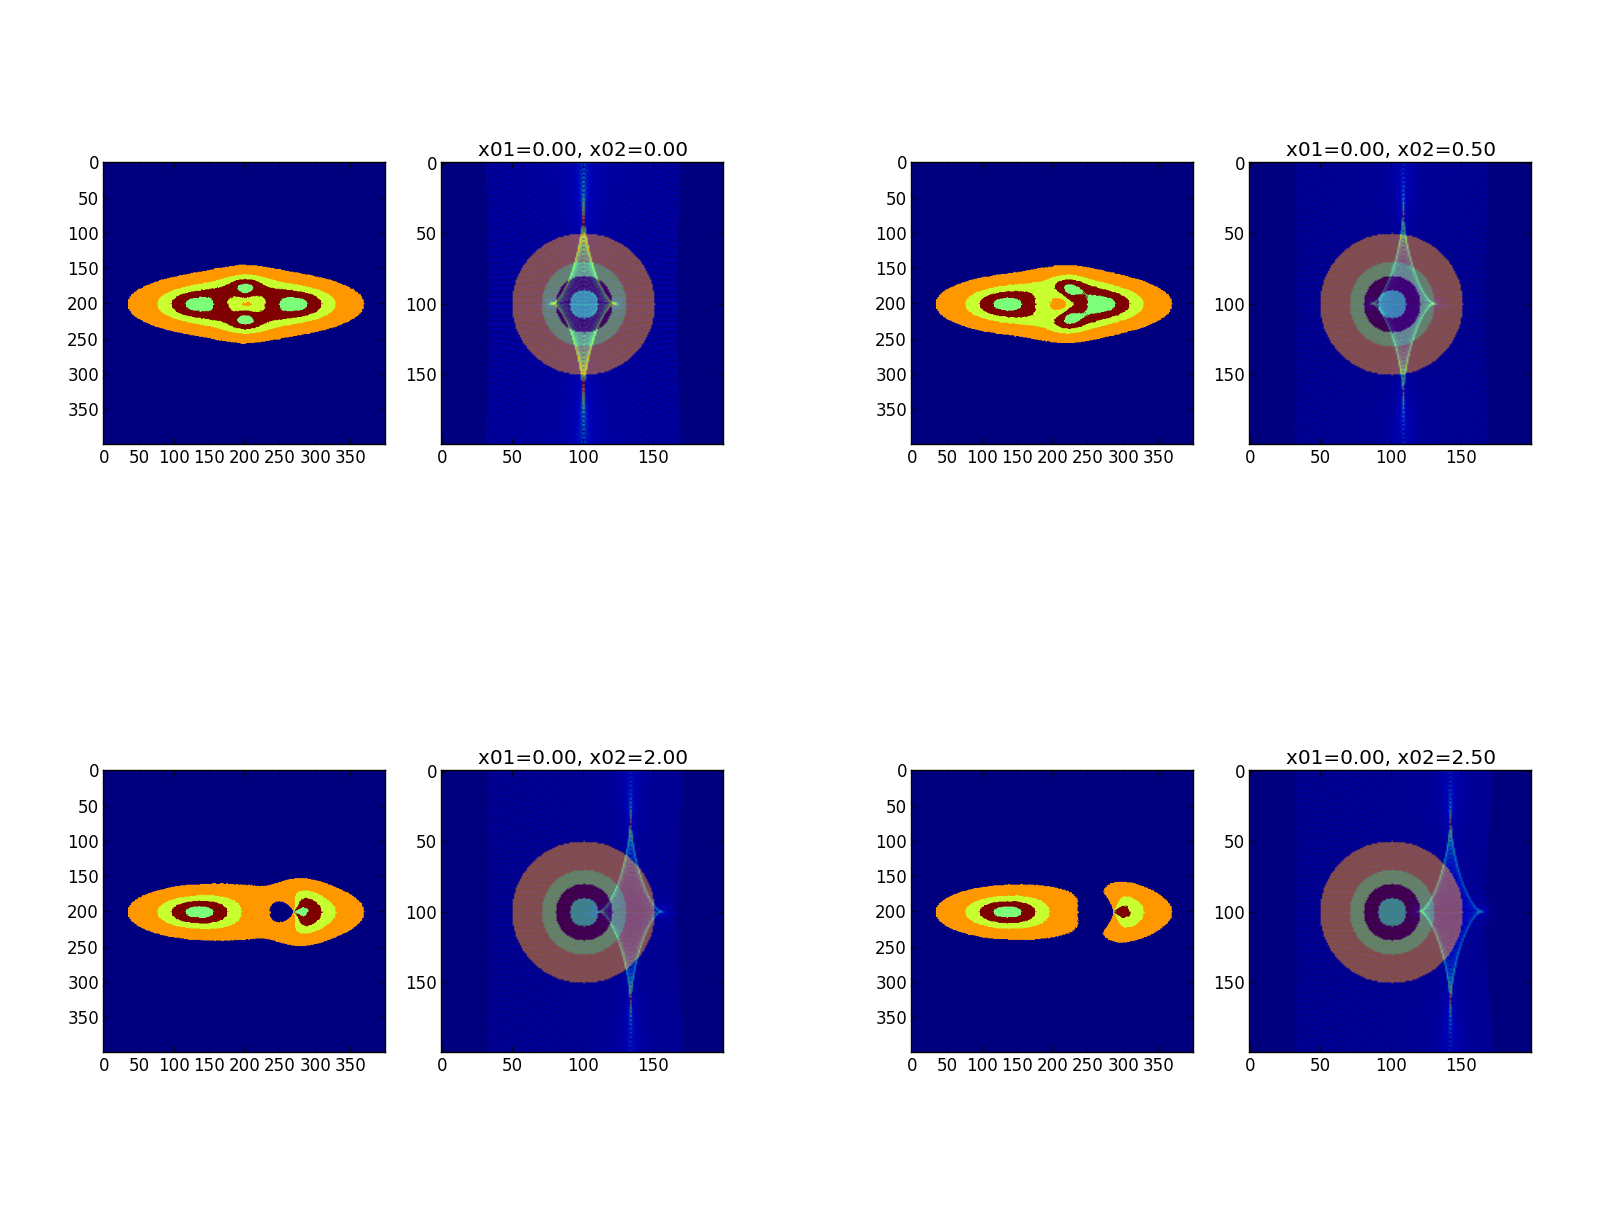
\includegraphics[scale=0.3]{caustic.png}
 \caption{\emph{SIS gamma = -0.5}}
 \label{Fig: 6}
\end{figure}

\end{document}

